
% V2.0 released 1998 December 18
% V2.1 released 2003 October 7 -- Gregor Hutton, updated the web address for the style files.

\documentclass{gji}
\usepackage{timet,color}
\usepackage[urlcolor=blue,citecolor=black,linkcolor=black]{hyperref}
\usepackage{fontsize}
\usepackage{fancyhdr}
\usepackage{amsmath}
\usepackage{graphicx}


\pagestyle{fancy}
\fancyhf{}
\fancyhead[L]{The ARTICLE ON MACHINE INTELLIGENCE and PATTERN ANALYSIS}
\fancyhead[R]{\thepage}

\renewcommand{\headrulewidth}{0pt} % Removes the horizontal line in the header

\let\leqslant=\leq

\newtheorem{theorem}{Theorem}[section]

\begin{document}

\begin{summary}
    \centering\fontsize{28}{32}\selectfont Enhancing Open Set Recognition through Metric Learning on Class-Specific Semantic Reconstruction Feature
\end{summary}

%\begin{writer}
    %\fontsize{12}{15}\selectfont Hongzhi Huang, Yu Wang, Qinghua Hu \textit{Senior Member, IEEE}, Ming-Ming Cheng \textit{Senior Member, IEEE}
%\end{writer}


\begin{abstract}
     \textbf{Abstract}---Metric learning (ML) is a type of machine learning. The ML goal is to learn a distance
function over objects. CSSR specifies metric learning for each known class as a substitute for the class-specific point set in the traditional prototype learning framework. Open set recognition enables deep neural networks (DNNs) to identify samples of unknown classes, while maintaining high classification accuracy on samples of known classes. In this study, we suggest a novel method, called Class-Specific Semantic Reconstruction (CSSR), that integrates the power of AE and prototype learning. In CSSR, prototype points are substituted with class-specific Autoencoders (AEs) that represent manifolds. Unlike traditional prototype-based methods, CSSR assigns each known class to a distinct AE manifold and evaluates class membership based on the AE's reconstruction error. These class-specific AEs are integrated into the top layer of the DNN backbone to reconstruct semantic representations acquired by the DNN, rather than the raw image data. By engaging in end-to-end learning, the DNN and AEs mutually enhance each other's ability to grasp both distinct and representative features. Experimental findings across various datasets demonstrate that this approach excels in both close and open set recognition tasks, offering a straightforward and adaptable integration into existing frameworks.
\end{abstract}

\begin{keywords}
    \textbf{Keywords}---Metric Learning, Open Set Recognition, Auto-encoder, Prototype Learning, Class-specific Semantic Reconstruction

    \centering
  \includegraphics[width=0.5\textwidth]{underline.png}
  
\end{keywords}


\section{Introduction} \label{section1}
\textbf{\textsc{Traditional}} deep neural networks (DNNs) are typically trained under the assumption that all test classes are familiar from the training phase. However, in real-world scenarios, test samples might belong to unfamiliar classes \cite {43}. When meeting such an unknown sample, traditional DNNs will compulsorily classify it as one of the known classes and make a wrong prediction, which may lead to irreparable losses in certain critical scenarios, such as medical diagnosis and autonomous driving.

Open set recognition (OSR) aims to address this issue by enabling models to accurately differentiate between samples from known (closed set) and unknown (open set) classes. One of the primary hurdles in OSR is the lack of information about unknown classes during training, making it challenging to distinguish between known and unknown classes and reduce the risk of misclassification.  \cite {34}. Traditional DNNs focus on learning discriminative features of known classes and partitioning the feature space accordingly. However, this approach often results in samples from unknown classes being misclassified as known classes with high confidence. \cite {42}. 

 In metric learning, the goal is to learn a distance function over objects. This is often used in tasks like image recognition, where the aim is to learn to identify similar images.
 As illustrated in Fig ~\ref{fig1}.,  the terms "positive", "negative", and "anchor" refer to specific types of images used in the learning process. These three types of images are used in a method called "tripletloss", where the aim is to make the distance between the anchor and positive images smaller than the distance between the anchor and negative images. This helps the model learn to accurately measure the similarity between images. \cite {10}.  Each image passes through a CNN and a AEs, that form the subnet, resulting in a features vector for each image. To verify the similarity, the Euclidean Distance between the vectors is calculated, passing through a Contrastive Loss function.The network receives as input a triplet given by anchor, positive and negative. Since the image identified by anchor is a reference image, positive is a different image, but the same person as the anchor and negative is a different person image. In this model, each subnet treats one of the input images and finally the network uses a Triplet Loss Function that attempts to bring the anchor closer to the positive and away from the negative so that re-identification can be performed.  \cite {10}. 
\begin{figure*}
\label{fig1}
 \centering
 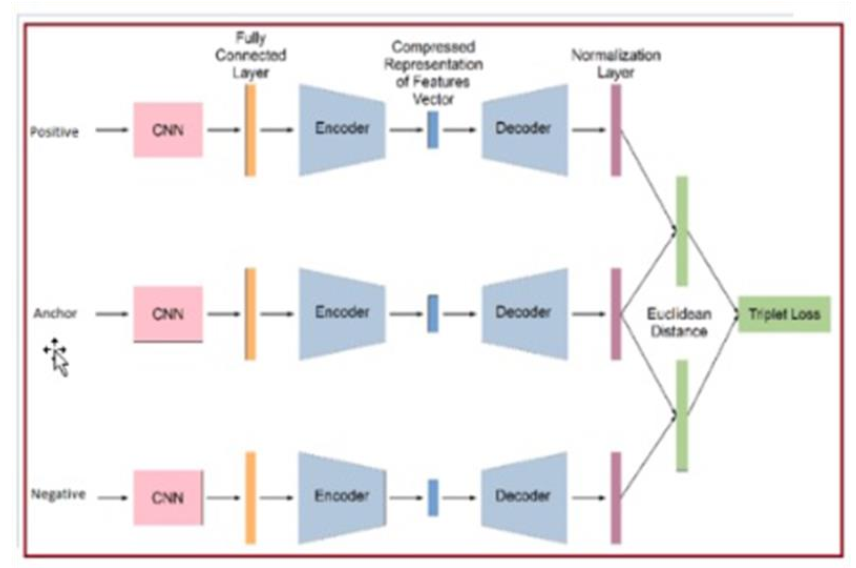
\includegraphics[width=0.48\textwidth]{fig1.png}
     \caption{Metric learning with CSSR}
   
\end{figure*}
 
 
 Prototype-like methods, such as generalized convolutional prototype learning and the recently introduced reciprocal point learning, differ from AE-based methods. These methods focus on learning specific points for each class to align with the extracted representations of the labeled class or the rest classes. The rationale behind these methods is clear, yet the prototype-learning framework encounters significant obstacles in the OSR task.   \cite {10},  \cite {36}. The primary challenge lies in the under-representation of classes, where a single point or a few points may not adequately represent the class. Prototype learning assumes a Gaussian distribution for class-specific features, which is often unrealistic in practical applications, leading to open space risk. Additionally, intra-class features are condensed into a limited number of points within prototype-learning frameworks, potentially causing the model to overlook essential information. 
 

Prototype-like methods, such as generalized convolutional prototype learning and the recently introduced reciprocal point learning, diverge from AE-based approaches\cite {4}. These methods focus on learning specific points tailored to the extracted representations of the labeled class or other classes. The rationale behind these techniques is clear-cut. Nevertheless, the prototype-learning framework encounters significant hurdles in the OSR task. The primary obstacle is the issue of class under-representation, where the use of a single point or a minimal number of points may not adequately capture the essence of the class. On one hand, prototype learning assumes a Gaussian distribution for class-specific features. However, this assumption is rarely met in real-world scenarios, leading to potential open space risk. \cite {42}. On the other hand, within prototype-learning frameworks, intra-class features are condensed into a limited number of points. This compression may result in the model filtering out crucial information necessary for distinguishing unknown classes. \cite {7}.

Our proposed framework offers a solution to the challenges highlighted in existing methods. In contrast to AE-based approaches, the CSSR method we introduce addresses these issues by (1) mitigating classification degradation through the elimination of redundant information and the reconstruction of semantic features rather than raw images, and (2) tackling the open space risk by acquiring knowledge of class-specific manifolds to unveil inter-class regions. In comparison to prototype-like techniques, our CSSR method effectively addresses the problem of class under-representation by mastering a class-specific manifold. This not only departs from the Gaussian assumption of classes but also preserves more essential class information than merely representing a class with a single point.

During the end-to-end learning process, the class-specific autoencoders and deep neural network mutually enhance each other to detect open space areas while acquiring highly class-specific semantic representations. The autoencoders are inclined to link each class with a particular set of semantic attributes. Instances of a known class typically activate relevant features while deactivating irrelevant ones. Conversely, for samples from an unknown class, their semantic features remain inactive as they do not correspond to any features of known classes. This characteristic is leveraged for identifying unknown classes. Results from experiments conducted across various datasets demonstrate that the proposed approach surpasses other cutting-edge methods significantly, enhancing the performance of both closed and open set recognition. In summary, this study presents the following contributions:

1) Our proposal introduces the CSSR method for open set recognition, a straightforward yet powerful approach. It assigns a dedicated autoencoder to each known class and integrates these autoencoders at the top of the DNN backbone to reconstruct the semantic representations acquired by the backbone network. CSSR enhances the fitting and learning capabilities, thereby boosting open set performance.

2) We provide a theoretical analysis to elucidate the open space risk associated with current methods and explore the links between CSSR and existing methodologies to gain a comprehensive understanding of CSSR.

3) Through experiments conducted under diverse protocols, we showcase that CSSR significantly outperforms baseline techniques and achieves top-tier performance on multiple public datasets. Notably, CSSR enhances the F1 score by an average of 8.3% in open set recognition tasks.


\section{\textbf \textsc{PPRELIMINARIES}}

\subsection{OOD Detection}

As initially proposed by Hendrycks and Gimpel \cite {15}, out-of-distribution (OOD) detection involves identifying samples that are not part of the training dataset. While various methods have tackled this issue with access to OOD samples during training  \cite {10}, \cite {21}, \cite {23},  \cite {31}, \cite {49}. Our focus lies on scenarios where only in-distribution data is available during training. While OOD detection can be simplified with known outliers, open set recognition is more practical and prevalent. Additionally, well-crafted models can benefit from exposure to outliers, such as OpenGAN \cite {19} which can operate with or without additional OOD data. In this discussion, we primarily concentrate on models trained without extra OOD data.

\textbf{Supervised Methods.} These approaches, akin to open set recognition, construct OOD detectors based on a classification task. Some methods aim to enhance score functions, such as maximizing SoftMax probability \cite {15}, maximum logit scores \cite {14}, and energy score \cite {23}. Vyas et al. \cite {40} employed an ensemble of leave-one-out classifiers to mimic individually accessible OOD training data. Sastry and Oore \cite{33} suggested characterizing activity patterns using Gram matrices and assessing OOD-ness by comparing element-wise deviations in the Gram matrices from the training data.

\textbf{Self-Supervised Methods.} These relatively new methods leverage well-learned representations through self-supervision. Golan and El-Yaniv \cite{11}, aalong with Hendrycks et al. [16], explored predicting image transformations (e.g., rotating images to 0°, 90°, 180°, and 270°), a task also used as an auxiliary task in \cite{38}. Self-supervised contrastive learning has
shown considerable success in unsupervised representation learning [5], [12], and is being applied to OOD detection \cite {38}. Self-supervised contrastive learning has demonstrated significant success in unsupervised representation learning \cite {5}, \cite {12}, and is being applied to OOD detection \cite {35}, \cite {38}, \cite {41}. Researchers have noted that representations obtained through contrastive learning exhibit distinct patterns between in-distribution and out-of-distribution data. Though initially designed for unlabeled scenarios, these methods have also been extended to supervised learning.

  
\subsection{Open Set Recognition}

Early studies employed traditional machine learning techniques, utilizing classifier scores to identify unknown samples by assessing their similarity to known classes \cite {1},  \cite {18}. For example, Scheirer et al. \cite {34} utilized a support vector machine for known class identification and applied the extreme value distribution to detect unknown samples. In recent times, deep neural networks (DNNs) have been leveraged for their strong representation learning capabilities in unknown sample detection. 

Numerous researchers have either developed or utilized the classification layer for open set recognition (OSR) \cite {15}, \cite {48}. A plain choice is to utilize the maximum SoftMax probabilities and reject unconfident predictions \cite {15}. Bendale et al. \cite {2} demonstrated the vulnerability of SoftMax probabilities and suggested replacing the SoftMax function with the OpenMax function, which redistributes SoftMax scores to explicitly derive the confident score of the unknown class. Zhou et al. [48] introduced the notion of placeholder learning, where overly confident predictions are adjusted by allocating classifier placeholders for unknown classes.

Given a set of n labeled instances, $X = \{f(x_i, y_i)\}_{i=1}^n$, where $y_i \in \{1, \ldots, m\}$ are the corresponding labels of known classes. 
For open set recognition, the objective is to train a model using dataset $X$ to categorize test samples into $m + 1$ classes, which include the $m$ known classes and an additional unknown class denoted by $m + 1$.

\textbf{Auto-Encoder}. An auto-encoder (AE) is designed to learn efficient representations of a dataset in an unsupervised manner.
By employing a bottleneck structure comprising cascaded encoder $f$ and decoder $g$, the AE is compelled to condense high-dimensional input features into a lower-dimensional embedding space H in order to accurately reconstruct the original input data. This process aims to minimize the reconstruction error $\lVert x - g(f(x)) \rVert^2_2$ for each input sample $x$. 

The decoder $g$ is responsible for learning a manifold $V = \{g(h) \mid h \in H\}$, whereas the encoder $f$ learns to map the original feature space to this manifold $V$. In open set recognition methods based on auto-encoders (AE), the manifold $V$ is aligned with the distribution of known class samples, with the reconstruction error serving as the distance metric between the input sample and the manifold $V$. Current approaches reconstruct the entire image and aim to minimize pixel-wise reconstruction errors. However, including background pixels (information irrelevant to the category) proves unproductive for both closed set and open set recognition. This inefficiency has been highlighted by Zhang et al. \cite{47}, who found that constructing a flow density estimator based on latent representations outperforms doing so directly on the raw image. Consequently, we construct AEs using the latent space derived from a backbone network.

\textbf{Prototype and Reciprocal Learning}. Prototype learning \cite{42} establishes class-specific points sets $U_i$ for each category $i$. In this approach, a test sample is assigned to the closest prototype point, while samples distant from all prototype points are identified as belonging to an unknown class. This method formally characterizes closed and open set recognition in the following manner:

\[
p(y = i \mid x, B, U) &\propto (- \min_{u \in U_i} \|B(x) - u\|_2^2), 
\]
\[
p(\text{unknown} \mid x, B, U) &\propto \min_i \min_{u \in U_i} \|B(x) - u\|_2^2, \tag{1}  \label{eq1} 
\]

where $B$ represents the backbone network responsible for extracting the embedding feature from input $x$. On the other hand, reciprocal learning (4) employs class-specific reciprocal point sets $U_i$ to understand otherness rather than belongingness. In this approach, samples in proximity to all reciprocal points are deemed unknown, as articulated by:

\[
p(y = i \mid x, B, U) &\propto \sum_{u \in U_i} \|B(x) - u\|_2^2,
\]
\[
p(\text{known} \mid x, B, U) &\propto \max_i \max_{u \in U_i} \|B(x) - u\|_2^2. \tag{2} \label{eq2} 
\]

During the training phase, the model focuses on optimizing the cross-entropy loss based on SoftMax normalized class probabilities. However, solely optimizing discriminative loss yields limited effectiveness. Consequently, both approaches introduce distinct regularization terms to address the challenges of open space risk and enhance training outcomes. Within the prototype framework, a generative loss $L_{pl}$ (also known as prototype loss) is introduced, serving as a maximum likelihood regularization assumption under the Gaussian mixture density framework:

\[
L_{pl}(x, y, U, B) = \min_{u \in U_y} \|B(x) - u\|_2^2 \tag{3} \label{eq3}
\]


For the reciprocal learning framework, open space risk is bounded by the constraining variance of feature-to-reciprocal point distances. This is formalized by
\[
L_{rp}(x, y, U, B) = \sum_{u \in U_y} \|d(B(x), u) - R_y|_2^2 \tag{4} \label{eq4} 
\]

where $d(\cdot, \cdot)$ is a distance function and $R_y$ is a class-specific learnable margin.

Both $L_{pl}$ and $L_{rp}$ impose additional compactness constraints. In this research, we note that optimizing a singular discriminative cross-entropy loss results in an incongruent distribution between feature distribution and prototype points. For further details, please see Section ~\ref{section4} for an in-depth discussion.

\section[]{\textbf\mdseries \textsc{M}\lowercase{\textsc{ethod}}} 

Prototype learning encounters two issues, as documented: (1) the fitting capacity of class-specific prototype point sets is limited, and (2) the lack of diverse representation hinders OSR. To enhance both the fitting and representation learning capabilities within the prototype-learning framework, we suggest harnessing the capabilities of Autoencoders (AEs), which create prototype manifolds to accommodate known classes. In this section, we initially present our primary architecture and examine how the proposed model addresses open space risk. Subsequently, we outline the proposed unknown detection strategy. Finally, we delve into the connections between our model and existing methodologies.


\subsection{Class-Specific Semantic Reconstruction}

We replace class-specific point set $U_i$ with an AE for each category $i$ denoted as $A_i$. As shown in Fig. ~\ref{fig2}, it takes a latent representation $z$ as input, and outputs the reconstructed representation $\hat{z} = A_i(z)$. Then, we calculate the reconstruction error by the L1-norm as

\[
d(z, A_i) = \|z - A_i(z)\|_{1}. \tag{5} \label{eq5}
\]

\begin{figure}  
\centering
  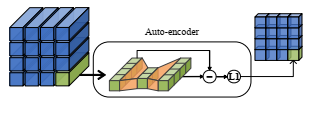
\includegraphics[width=0.48\textwidth]{fig2.png}
     \caption{Structure of individual AEs. Note that we operate the reconstruction process at the pixel level. It takes the semantic feature map as input and outputs the reconstruction error at each pixel.
.} \label{fig2}
    
  \end{figure}

After prototype learning, our framework can estimate class membership based on the reconstruction error.
Given sample $(x, c) \in X$, we let $p(y = j|x) &\propto (-d(z, A_i))$ to learn the prototype manifold. By applying SoftMax to normalize the logits, the final probability can be defined as
\[
p(y = j|z, A) = \frac{e^{-\gamma d(z,A_i)}}{\sum_{j=1}^{m} e^{-\gamma d(z,A_j)}}, \tag{6} \label{eq6} 
\]

In this context, $\gamma$ represents a hyperparameter that governs the level of difficulty in assigning probabilities. In striving for an optimal solution that maximizes the output probability for the true category, the Autoencoders (AEs) should initially learn a mapping of minimal distance (from feature to manifold) to reduce the reconstruction error for the true category. Simultaneously, the manifolds of the AEs should also learn to maintain a distance from each other to increase the reconstruction error for all AEs except the one corresponding to the true category.

As outlined in the introductory section, each class-specific AE $A_i$ defines a class-specific manifold $V_i$. Under the aforementioned ideal conditions, maximizing $p(y = c|j,x, A)$ can be viewed as prototype learning with an infinite number of prototype points (manifold $V_i$). Assuming that $d(z, A_c)$ is minimized, the reconstruction error can be approximated as:

\[
d(z, A_c) = \|z - A_c(z)\|_{1} \approx \min_{v \in V_c} \|z - v\|_{1}. \tag{7} \label{eq7} 
\]
This process of point assignment is equivalent to (~\ref{eq1} ), with point set $U_c$ replaced by $V_c$ and the squared L2-norm replaced by the L1-norm.

\subsection{Managing Open Space Risk}
\subsubsection{Fitting Known Classes} \label{section4} 
In prototype point learning, the mean square error (MSE) serves as the distance metric. It is noted that utilizing MSE may lead to learning an inconsistent distribution between prototype points and semantic features.

The prototype loss, as defined in Eq. (\ref{eq3}), functions as a regularization term within GCPL, aiming to directly diminish this gap and effectively address the open space risk. Subsequently, we will delve into an analysis of how MSE contributes to the mentioned inconsistency, contrasting with the mean absolute error utilized in Eq. (\ref{eq5}), which maintains consistency.

In our analysis, we focus on the most basic form of prototype learning, where $|U_i| = 1$ and $u_i \in U_i$ denotes the sole prototype point for class $i$. Consequently, $d(z, U_i)$ simplifies to $\|z - u_i\|$, and the SoftMax probability for category $i$ is calculated as:

\[
p(y = i|z, U) = \frac{\exp(-\|z - u_i\|)}{\sum_{j} \exp(-\|z - u_j\|)}. \tag{8} \label{eq8} 
\]

By examining $z = u_c + \epsilon$, we investigate how $p(y = c|z, U)$ changes as $\epsilon$ varies when employing MAE and MSE. The objective of prototype learning is to maximize $p(y = c|z, U)$ when a sample precisely aligns with its prototype point, i.e., $z = u_c$. The probability should decrease as the deviation $\epsilon = z - u_c$ increases. However, the subsequent theorems demonstrate that this objective cannot be attained when utilizing MSE.

Theorem 1. With $d(z, U_i) = \|z - u_i\|_2^2$, assuming $u_i \neq u_j$ for $i \neq j$, there exists $c$ and $\epsilon \neq 0$ satisfying $p(y = c|u_c, U) < p(y = c|u_c + \epsilon, U)$.

Theorem 2. With $d(z, U_i) = \|z - u_i\|_1$, for each $c$, $\epsilon$, $p(y = c|u_c, U) \geq p(y = c|u_c + \epsilon, U)$ stands.


The proofs for the two theorems are available in the supplementary file. Assuming $c$ is the label corresponding to $z$, Theorem 1 suggests that when using MSE, $z = u_c$ might not be the optimal solution for maximizing $p(y = c|z, U)$ and minimizing the cross-entropy loss, leading to the aforementioned inconsistent distribution. On the other hand, as per Theorem 2, MAE ensures that $p(y = c|u_c, U) \geq p(y = c|u_c + \epsilon, U)$, guaranteeing maximum $p(y = c|j,z, U)$ and minimal cross-entropy loss when $z = u_c$. This alignment ensures consistency between the distributions of the semantic feature and prototype point. The experiment depicted in Fig. ~\ref{fig3} demonstrates well-fitted prototypes and effective management of open space risk.

The proofs for the two theorems are available in the supplementary file. Assuming $c$ is the label corresponding to $z$, Theorem 1 suggests that when using MSE, $z = u_c$ might not be the optimal solution for maximizing $p(y = c|z, U)$ and minimizing the cross-entropy loss, leading to the aforementioned inconsistent distribution. On the other hand, as per Theorem 2, MAE ensures that $p(y = c|u_c, U) \geq p(y = c|u_c + \epsilon, U)$, guaranteeing maximum $p(y = c|j,z, U)$ and minimal cross-entropy loss when $z = u_c$. This alignment ensures consistency between the distributions of the semantic feature and prototype point. The experiment depicted in Fig. ~\ref{fig3} demonstrates well-fitted prototypes and effective management of open space risk.

\begin{figure}  
\centering
  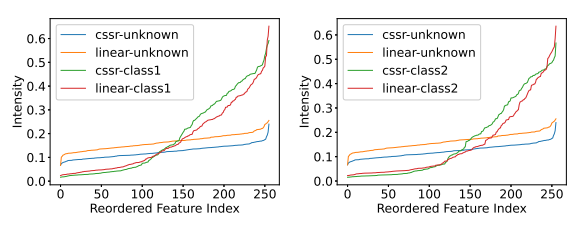
\includegraphics[width=0.48\textwidth]{fig4.png}
     \caption{Displaying the class-specific feature activation for CSSR involved selecting six categories from Cifar10 as known classes and considering the remaining four as unknown. It's important to mention that the magnitude of each feature is standardized across the six known classes, and we arranged each curve in ascending order to enhance the clarity of visualization..
} \label{fig3}
    
  \end{figure}


\subsubsection{Learning Class-Related Features}
In the process of jointly optimizing the backbone network and class-specific AEs, learning occurs on both fronts. Not only are the AEs trained to match known classes, but the backbone network is also trained simultaneously to align the extracted features with the class-specific characteristics. This approach tackles the challenges outlined in Section ~\ref{section1}, emphasizing the need for diverse and well-learned representations. The inherent diversity is reflected in features situated on the manifold surface. Additionally, the reconstruction error in the vertical direction of the manifold encourages a compact representation, leading to semantic features that are closely tied to specific classes. Each category is defined by a subset of global features, with samples predominantly activating features associated with their respective categories.

To illustrate the concept of learning class-specific features more easily, let's consider a scenario where the AEs are simplified: each encoder functions as an identity mapping for a class-specific feature subset, and the decoder mirrors this mapping. When activating features relevant to a class, no reconstruction error occurs; however, activating non-related features results in errors. To minimize these errors, the backbone network learns to activate only class-related features. By employing joint optimization, the backbone network acts as a robust fit, simplifying the AE's task. Ultimately, this model excels at extracting class-specific features, a capability that can also be utilized for detecting unknown classes, as discussed later in this section. ~\ref{section4.4}

Figure ~\ref{fig3} illustrates the average intensity of activation (absolute activation value) for both known and unknown classes. Known classes exhibit strong activation on specific features while showing minimal activation on others. In contrast, unknown classes display low activation across all features since they lack training and association with specific features. The features extracted by CSSR offer several advantages over a plain linear classification layer: (1) class-related features in CSSR contribute more uniformly across features rather than focusing on a select few, (2) class-unrelated features in CSSR are less activated, and (3) the activation intensity for unknown classes in CSSR is notably lower than that of a standard linear classifier, indicating a stronger connection between known classes and learned semantic features.

A recent novelty detection method based on representation learning \cite{38} observed that a well-learned representation enables direct differentiation of feature magnitudes between in-distribution and out-of-distribution (OOD) data. Furthermore, addressing the challenge of OOD data availability during training, Dhamija et al. \cite{9} proposed a loss function to explicitly reduce the activation magnitude for OOD data. Remarkably, for CSSR, this characteristic is inherently fulfilled without the need for OOD data during training.
  
  
\subsection{Overall Framework}
Figure ~\ref{fig5} depicts the training and inference processes for the proposed approach. The framework consists of two primary components: a backbone network $B$ responsible for acquiring latent representations and class-specific AEs utilized for classifying known classes and identifying unknown classes.

In order to maximize the utilization of the semantic feature map $Z = \{z_{ij}\}$ obtained from $B$, we assign equal importance to the latent representation of each pixel. Subsequently, we generate a global prediction by averaging the predictions made at the pixel level:

\[
p(y = i|Z, A) = \frac{1}{|Z|} \sum_{z \in Z} p(y = i|z, A). \tag{9} \label{eq9} 
\]

Apparantly, $p(y = i|Z, A)$ sums to one, as $p(y = i|z, A)$ sums to one individually. Finally, the model is trained by minimizing the negative log-probability of the true class $c$ via gradient descent as follows:

\[
L = -\log p(y = c|Z, A). \tag{10} \label{eq10} 
\]

Since each pixel's representation focuses on a local part of the input image, these operations can be seen as enhancing the raw input through soft cropping and combining the prediction results of augmented images. During testing, this method naturally incorporates test augmentation techniques, leading to improved performance. These operations can be executed using 1 × 1 convolutions, pixel-wise SoftMax, and global average pooling. Additionally, the AEs are implemented with a simple linear encoder and decoder utilizing the tanh activation function and no bias.

Building on the concept introduced in \cite{4}, the proposed approach can be expanded into a reciprocal learning framework. Here, the class-specific AEs can estimate otherness instead of reciprocal point sets. The only adjustment required is the introduction of a negative hyperparameter $\gamma$. Subsequently, akin to Eq. (~\ref{eq7}), assuming maximization of $d(z, A_c)$, the reconstruction error can be approximated as:

\[
d(z, A_c) = \|z - A_c(z)\|_{1} \approx \max_{v \in V_c} \|z - v\|_{1}. \tag{11} \label{eq11}
\]

This process is equivalent to Eq. (~\ref{eq7}). We refer to the reciprocal version of CSSR as RCSSR in the rest of this paper.

\begin{figure*}
\label{fig5}
 \centering
  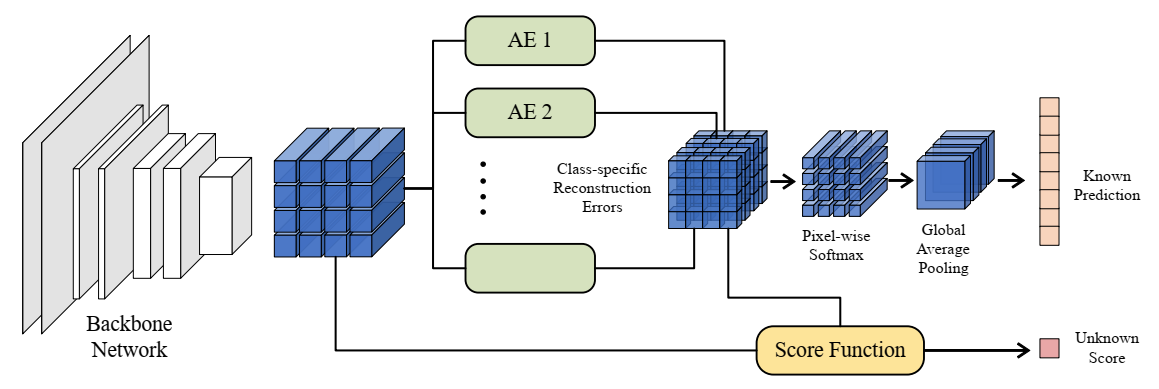
\includegraphics[width=1\textwidth]{fig5.png}
     \caption{The foundational structure of our proposed model involves the backbone network ($B$) processing an image to derive its semantic feature map $z$. The class-specific AE ($A_c$) associated with class $c$ encodes and reconstructs the pixel-wise semantic representation $z$. Following this, we utilize the pixel-wise reconstruction errors from the class-specific AEs as logits, which are then subjected to pixel-wise SoftMax after being multiplied by $\gamma$. Subsequently, global average pooling is employed to condense the pixel-wise predictions into an overall prediction for the entire image.
    During unknown inference, the model leverages the pixel-wise reconstruction errors linked to the predicted class along with the semantic features as input to assess the unknownness of the image. Finally, a threshold is established to ensure that 95\% of known samples are correctly identified; samples with unknown scores below the threshold are rejected.
    } \label{fig5}
   
\end{figure*}

\subsection{Detecting Unknown Classes} \label{section4.4}
  \subsubsection{Reconstruction Error-based Score Function}
    An intuitive approach is to leverage the reconstruction error for detecting unknown classes. As discussed in Section 4.2.2, unknown samples result in inactive semantic features. We have noticed that poorly activated semantic features lead to low reconstruction errors, which can hinder the detection of unknown classes.
    
    Given that we employ AEs with a linear decoder and a linear encoder activated by $\tanh$, we consider the approximate linear relationship between $|z|{1}$ and $|z - A{c}(z)|_{1}$. The encoder $f$ and decoder $g$ adhere to the properties of linear functions, where $f(\lambda z) = \lambda f(z)$ and $g(\lambda z) = \lambda g(z)$. With the $\tanh$ activation, $\tanh(\lambda z) \approx \lambda \tanh(z)$ under the assumption that $f(z)$ is centered around zero. Consequently, this leads to:
  
    \[
    \| \lambda z - A_{c}(\lambda z) \|_{1} \approx \lambda \|z - A_{c}(z)\|_{1},
    \]
    
    and To eliminate the scaling factor $\lambda$, we divide by $|z|{1}$. Ensuring that $z$ is centered around zero is straightforward for unknown samples. Additionally, we enhance the unknown detection capability of feature magnitude by introducing an additional term $|z|{1}$.
    In particular, we define the first score function as follows: Known classes in CSSR are expected to exhibit a low relative reconstruction error while demonstrating high feature magnitude. This is given by
    \[ s_{p1}(z, c) = -\frac{d(z, A_c)}{\|z\|_{2}^{1}}. \tag{12} \label{eq12} \]
    Meanwhile for RCSSR, known class samples should have high relative reconstruction error and high feature magnitude:
    
    \[ s_{r1}(z, c) = \frac{d(z, A_c)}{\|z\|_{1}} \times \|z\|_{1} = d(z, A_c). \tag{13} \label{eq13} \]

    Just like the closed-set classification procedure, where pixel-wise features are maximally utilized, we evaluate the feature map $Z$ on a pixel-by-pixel basis. The individual scores are aggregated to form the final score for the entire image, denoted as $s^*(Z, c) = \frac{1}{|Z|} \sum_{z \in Z} s^*(z, c)$, where $s^*$ can be either $s_p^1$ or $s_r^1$ (Please note that $^*$ denotes the selection of CSSR or RCSSR).

    In contrast to the original prototype learning approach, $s_p^1$ varies due to its representation learning capability. On the other hand, $s_r^1$ maintains the same structure as Eq. (\ref{eq2}) in reciprocal learning, incorporating the approximation in (\ref{eq11}) and the prediction function $c = \arg \max_i d(z, A_i)$.

  \subsubsection{Activation Pattern-based Score Function}

    Assume that the semantic feature map $Z_i$ and predicted class $c_i$ are derived from sample $x_i$ in the training set. Since our focus lies solely on the activation intensity of the features, we preprocess all feature maps by computing the absolute values of their elements. For the purposes of our discussion, we assume that the feature map has undergone preprocessing. To fulfill the need for class-specific patterns, the feature maps are categorized into distinct sets based on their predicted classes, i.e., feature sets $Z_c = \{Z_{i} | c_i = c, i = 1, 2, \ldots, n_c, c = 1, \ldots, m\}$.

    For the first-order statistics, we first take the class-specific mean activation intensity:
    
    \[ \mu_i =  \sum_{z \in Z^i} \sum_{z \in Z} \frac{1}{|Z^i| |Z|} z. \tag{14} \label{14} \]
    
    To consider the different scales of the activation intensities for different features, a normalization cross categories is further applied:
    
    \[ \tilde{\mu}_i = \frac{\mu_i}{\sum_{j} \mu_j}, \tag{15} \label{eq15} \]
    
    where the vector division is conducted elementwise.
    
    To detect unknownness, a sample activating what a known class activates is more likely to be the same known class. Specifically, the activation intensity of each feature is weighed by $\tilde{\mu}_c$, and the unknownness is evaluated by the weighted average intensity across features. Pixel-wise score integration is performed as well. Formally, the score function is defined by
    
    \[ s^2(Z, c) = \sum_{z \in Z} \frac{1}{|Z|} z^T \cdot \tilde{\mu}_c. \tag{16} \]

    Drawing inspiration from Sastry and Oore \cite{33}, we employ Gram matrices to capture inter-feature co-occurrence for second-order statistics. Let $F \in \mathbb{R}^{D \times |Z|}$ represent the feature intensity matrix, where pixel-wise vectors from the feature map $Z$ are concatenated column-wise, and $D$ denotes the feature dimension. The Gram matrix for the $i$th sample is formulated as $G = FF^T$. Within a Gram matrix $G$, the elements signify the likelihood of simultaneous activation between the respective two features (indexed by row and column).

    To model feature co-occurrence patterns, we compute the average Gram matrices specific to each class from the feature maps. These matrices serve as templates for inter-feature relationships. Subsequently, for a test sample, we compute its Gram matrix and evaluate its unknownness by summing the element-wise products with the precomputed template corresponding to its predicted label. This process can be expressed as:
    
    \[ G^c = \frac{1}{|Z^c|} \sum_{Z \in Z^c} G(Z), \tag{17} \label{17} \]

    \[ s_3(Z, c) = \text{Sum}(G^c \odot G(Z)), \tag{18} \label{18} \]

In this context, $\text{Sum}(\cdot)$ denotes a function that aggregates matrix elements, and $\odot$ signifies element-wise matrix multiplication. We observe that the aforementioned operation is akin to expanding the pixel-wise feature $z$ into a second-order polynomial space, specifically $zz^T = [z_iz_j]_{D \times D}$. The Gram matrix can be expressed as the summation of pixel-wise extended features, denoted as $G = \sum_{z \in Z} zz^T$, where $G_c$ signifies the first-order statistics within the extended feature space.

\[ s_3(Z, c) = \sum_{z \in Z} \text{Sum}(G^c \odot zz^T). \]

In addition to the primary definition of Gram matrix, the extended higher-order Gram matrix proposed in \cite{33} is optional here, i.e.,

\[ G = \left( F^p(F^p)^T \right)^{\frac{1}{p}}, \tag{19} \label{19}  \]

where the power on matrix is calculated element-wise. We found that the higher-order Gram matrix marginally improves the performance, we set $p = 8$ by default in the rest of this paper.

  \subsubsection{Integrated Score Function}

  Prior to consolidating the scores mentioned above, we conduct a normalization step on individual scores to ensure uniform scaling across different score functions. To achieve this, we derive scores for random augmented training samples for each score function $s^*$ to mitigate the impact of overconfidence stemming from well-fitted training samples. Subsequently, we calculate the mean and standard deviation, which are then utilized for normalization purposes. The process can be expressed as

    \[ \tilde{s}_*(Z, c) = \frac{s_*(Z, c) - E(s_*)}{\text{Std}(s_*)}, \tag{20} \label{eq20} \]
    
    where $E(s^*)$ and $\text{Std}(s^*)$, respectively, represent the precomputed mean and standard deviation with respect to $s^*$. We now integrate all three score functions via a linear combination to obtain our final score function:
    
    \[ s_{\text{all}}(Z, c) = w_1 \times \tilde{s}_*1(Z, c) + w_2 \times \tilde{s}^*_2(Z, c) + w_3 \times \tilde{s}^*_3(Z, c), \tag{21} \label{eq21} \]

    where $s^*_1$ represents either $s_p^1$ or $s_r^1$, and $w_1$, $w_2$, and $w_3$ are weights for each detection score.
    

    
    The process is illustrated in Fig. ~\ref{fig6}. We summarize our procedure for unknown detection as follows: (1) Run over the training set without data augmentation to collect first-order and second-order statistics on semantic features. This step using non-augmented training samples preserves complete information for known classes. (2) Run over the training set with data augmentation to collect the normalization parameters for individual scores. This step using augmented training samples reduces the effect of overconfidence. (3) Make inference using the integrated score in Eq. (~\ref{eq21}). To reject unknown class samples, we take a threshold that guarantees 95\% known samples being accepted.

\subsection{Connection to AE-based Methods}

AE-based open set recognition methods \cite{26}, \cite{27}, \cite{36} involve simultaneous learning of the classification and reconstruction tasks within the model. Recent advancements have pursued this objective through either multi-task learning or multi-stage learning strategies. In addition to addressing the challenges posed by AEs, as discussed in Section 4.2, we evaluate existing methods from a training framework perspective.

Multi-task learning \cite{27}, \cite{36} aims to jointly optimize the classification and reconstruction tasks by leveraging shared knowledge to develop a unified representation. Consequently, these methods may exhibit slightly lower performance in closed-set classification compared to straightforward classification approaches. On the other hand, the multi-stage approach \cite{26} entails training an encoder for a classification task initially, followed by training the decoder while keeping the encoder parameters fixed. While this strategy can maintain closed-set performance, it may encounter difficulties in decoder training due to the encoder's focus on extracting discriminative classification features, which may not contain sufficient information for detailed reconstruction.

As discussed in Section ~\ref{section1}, separating the close-set classification and image-reconstruction tasks can constrain performance as the encoded background information may impede the classification task, necessitating a trade-off between the two tasks. The proposed method addresses these challenges through two key strategies:

(1)CSSR reconstructs semantic features rather than the raw image, thereby avoiding unnecessary background pixel reconstruction and focusing on representative class-related semantic features.
(2)CSSR integrates the reconstruction and classification tasks, with the reconstruction task trained based on classification loss. This approach fosters a positive correlation between the performance of the two tasks instead of necessitating a trade-off.


\section[]{\textbf\mdseries \textsc{E}\lowercase{\textsc{XPERIMENTS}}} 

\subsection{Implementation Details}
    Since CSSR only modifies the classification layer, a variety of backbone networks can be employed to implement CSSR. Consistent with Chen et al. \cite{4}, we opted to train small-scale datasets using a Wide-ResNet (WRN40-4) \cite{45} with a depth of 40, width of 4, and dropout rate of 0. However, for larger-scale datasets like TinyImageNet, we switched to using ResNet18 \cite{13} for improved efficiency. During training, we utilized the stochastic gradient descent optimizer with a momentum of 0.9, training the model for 200 epochs with a fixed batch size of 128. The initial learning rate was set to 0.4, subsequently decreasing by a factor of 10 at the 130th and 190th epochs. The absolute value of the hyperparameter γ was set to 0.1 for all experiments.

    The AEs were constructed with linear encoders and decoders, employing the tanh activation function to ensure that the embedding space H remains bounded. The dimension of the embedding space for AEs was established at 64 for both the ResNet18 and WRN40-4 architectures. The integration weights for score integration were uniformly set to 1.

     \begin{table*}
 \begin{minipage}{115mm}
\centering
\caption{AUROC comparison between different methods on unknown detection tasks. }
\label{anymode}
\begin{tabular}{|@{}l|l|l|l|l|l|} \hline  
Methods& SVHN& CIFAR10& CIFAR+10& CIFAR+50& T\\ \hline  

CROSR\cite{10}& 89.9& 88.3&
  91.2& 90.5& 58.9\\[2pt] \hline  
 ARPL\cite{10}& 96.7& 91.0& 97.1& 95.1&78.2\\ \hline  
C2AE\cite{26}& 92.2&89.5&
  95.5& 93.7& 74.8\\[1.5pt] \hline  
MLOSR\cite{27}& 95.5& 84.5&
  89.5& 87.7& 71.8\\[1.5pt] \hline  
CFROSR\cite{28}& 93.5& 83.1&
  91.5& 91.3& 64.7\\[1.5pt] \hline  
PROSER\cite{48}& 94.3& 89.1&
  96.0& 95.3& 69.3\\[1.5pt] \hline  
CSSR& \bf{98.1}& 91.3&
  96.2& \bf{97.8}& \bf{84.5}\\[1.5pt] \hline  
RCSSR& 96.8& \bf{92.3}&
  95.7& 97.2& 83.1\\[1.5pt] \hline 
\end{tabular}

\end{minipage}
\end{table*}
    
    To enhance open set discrimination, previous methods have utilized data augmentation techniques. Following the methodology outlined in prior studies \cite{28}, \cite{48}, we applied a simple data augmentation technique introduced in \cite{8}. This technique involves considering a subset of transformations from RandAugment, including Brightness, Color, Equalize, Rotate, Sharpness, Shear, and Contrast. For each input image, up to two of these transformations are randomly selected and applied.
    
    In addition to prototype CSSR, we also implemented and evaluated RCSSR to provide a comprehensive comparison between the two methods.



\subsection{Comparison with State-of-the-art Results}
\subsubsection{Unknown Detection}
The evaluation protocol outlined in \cite{24} was utilized. This study involved five image datasets: SVHN \cite{25}, TinyImageNet \cite{30}, CIFAR10 \cite{20}, CIFAR+10, and CIFAR+50. For SVHN and CIFAR10, six classes were randomly chosen as known classes, while the remaining four classes were designated as unknown classes. In the case of TinyImageNet, 20 classes were selected as known classes, with the remaining 180 classes categorized as unknown. In the CIFAR+M datasets, the model was trained on four non-animal classes from CIFAR10 as known classes, while M animal classes from the CIFAR100 dataset \cite{20} were randomly assigned as unknown classes.

The evaluation metric used was the area under the receiver operating characteristic (AUROC) curve, a threshold-independent measure. The AUROC value reaches "1" when knowns and unknowns are entirely separable. By varying thresholds and plotting the true positive rate against the false positive rate, the AUROC was computed. Consistent with [24], the results were averaged across five randomized trials.

In comparing our method to related frameworks, including AE-based methods \cite{26} and prototype-like methods \cite{3}, \cite{42}, as well as two recent methods [24], [48] employing different architectures, the results are detailed in Table 1; values other than CSSR were sourced from \cite{48}. CSSR outperformed all other approaches across the five datasets, with slight performance lagging behind ARPL on CIFAR+10. Notably, CSSR demonstrated superior performance on SVHN (+1.4\%), CIFAR+50 (+1.3\%), and TinyImageNet (+4.6\%).

\subsubsection{Open Set Recognition}
Aside from identifying unknown classes, open set recognition necessitates the simultaneous classification of known classes while distinguishing and rejecting the unknowns. We adopted the experimental setup proposed by Yoshihashi et al. \cite{10}, wherein the models were trained on the complete CIFAR10 dataset as known classes. During the testing phase, samples from other datasets, such as ImageNet \cite{32} and LSUN \cite{44}, were utilized as unknowns. These datasets were either cropped or resized to match the same image size as the known samples. Specifically, 10,000 samples were selected to align with the CIFAR10 test set, forming ImageNet-Crop (IMGNC), ImageNet-Resize (IMGN-R), LSUN-Crop (LSUN-C), and LSUN-Resize (LSUN-R). To ensure fairness in comparison, we utilized the dataset versions released by Liang et al. \cite{22}.

Performance evaluation was conducted using macro-averaged F1-scores across 11 classes (comprising 10 known classes and 1 unknown). The results are detailed in Table 2, with values for CSSR sourced from \cite{36}. Notably, CSSR models demonstrated significantly superior performance compared to existing methods, showcasing an average improvement of 8.7\%.

     \begin{table}
 \begin{minipage}{65mm}
\caption{Open set classification results on the CIFAR-10 dataset with various unknown datasets added in the test phase}
\label{anymode}
\begin{tabular}{|@{}l|l|l|l|l|} \hline  
Methods& IMGN-C& IMGN-R& LSUN-C& LSUN-R\\ \hline  

Plain Softmax& 63.9& 65.3&
  64.2& 64.7\\[2pt] \hline  
C2AE\cite{26}& 83.7&82.6&
  78.3& 80.1\\[1.5pt] \hline  
CROSR\cite{10}& 72.1& 73.5&
  72.0& 74.9\\[1.5pt] \hline  
CFROSR\cite{28}& 75.7& 79.2&
  75.1& 80.5\\[1.5pt] \hline  
PROSER\cite{48}& 84.9& 82.4&
  86.7& 85.6\\[1.5pt] \hline  
CSSR& 93.2& 91.5&
  \bf{95.2}& 93.5\\[1.5pt] \hline  
RCSSR& \bf{94.5}& \bf{91.8}&
  94.1& 94.6\\[1.5pt] \hline 
\end{tabular}

\end{minipage}
\end{table}
    
\subsubsection{OOD Detection}  

 In this section, we followed the experimental setup outlined by Chen et al. \cite{3} to conduct a comparison with methods in an Out-of-Distribution (OOD) detection scenario. Additionally, we evaluated CSI \cite{38} and OpenGAN \cite{19} in this study. CSI adopts a similar approach of utilizing well-learned image representations for OOD sample detection. To ensure a fair comparison, we disabled the test augmentation technique for CSI during the evaluation process.

For OpenGAN, we employed the backbone trained in our baseline model as its feature encoder and directly utilized the corresponding test unknown dataset as its OOD validation set for model selection. The evaluation encompassed two challenging pairs of OOD detection benchmarks \cite{15}, involving three common datasets: CIFAR10, CIFAR100, and SVHN. The models were trained on CIFAR10, with CIFAR100 and SVHN serving as the near OOD and far OOD datasets, respectively, during the testing phase. It is important to note that overlapping categories were excluded from CIFAR100.

In addition to the Area Under the Receiver Operating Characteristic (AUROC), we incorporated several other evaluation metrics as per the methodology described by Chen et al. \cite{3}.

\subsection{Ablation Study}
In this section, we delve into the analysis of the contributions stemming from various components and score functions of CSSR. Initially, we conduct a comparison of different architectures for the model.

Datasets: Our models were trained on CIFAR10, with all 10 classes in CIFAR10 utilized as known classes for experimentation. Subsequently, testing was carried out on SVHN, LSUN-Resize, ImageNet-Resize, LSUN-Fix (LSUN-F), and ImageNet-Fix (IMGN-F). LSUN-Fix/ImageNet-Fix comprises randomly sampled and resized images from LSUN/ImageNet as generated by Tack et al. \cite{38}, rendering these datasets more challenging compared to the original versions released by Liang et al. \cite{22}.

Classification Layer: We compared traditional classification models with plain linear classification layers as baselines, maintaining the backbone and hyperparameters constant for equitable comparison.
Classification Strategy: We employed the proposed pixelwise prediction strategy (pixelwise SoftMax; then average pooling, denoted as SM-AP) or the plain prediction strategy (average pooling; then SoftMax, referred to as AP-SM). The pixelwise prediction strategy impacts both training and testing.
Reconstruction Error Measurement: Reconstruction errors were quantified using Mean Squared Error (MSE) or Mean Absolute Error (MAE) by default for CSSR.
The outcomes are summarized in Table 4, indicating the following: (1)CSSR, as a non-linear classification layer, marginally enhances closed-set performance.
(2)Pixelwise classification yields slight improvements in closed-set classification performance while significantly enhancing unknown detection performance.(3)Employing MAE as a distance measure generally outperforms MSE, underscoring MSE as a preferable choice for detecting unknown samples.

     \begin{table*}
 \begin{minipage}{115mm}
\centerin1
\caption{Ablation study on various architectures. The first row specifies the datasets used as unknown classes; ”Close Acc” represents closed set test accuracy (\%). For unknown detection, we provide AUROC values for evaluation. 

  }
\label{anymode}
\begin{tabular}{|@{}l|l|l|l|l|l|l|l|} \hline  
Methods& Close Acc& SVHN& LSUN-R& LMGN-R& LSUN-F & IMGN-F&Average\\ \hline  

Linear& 96.77& 97.0&
  95.2& 94.2& 92.3& 93.2&94.4\\[2pt] \hline  
 Linear SM-AP& 96.96& 96.8& 95.7& 94.8&92.9& 93.4&94.7\\ \hline  
CSSR AP-SM& 96.96&98.9&
  98.5& 97.1& 89.7& 89.5&94.7\\[1.5pt] \hline  
CSSR MSE& 96.85& 98.9&
  98.5& 97.3& 95.4& 94.4&96.9\\[1.5pt] \hline  
CSSR& 96.86& 99.1&
  98.8& 97.5& 96.2& 95.3&97.4\\[1.5pt] \hline  
RCSSR AP-SM& 96.84& 97.4&
  97.1& 95.5& 88.1& 89.2&93.5\\[1.5pt] \hline  
RCSSR MSE& 96.82& 98.7&
  97.8& 96.5& 92.0& 91.1&95.2\\[1.5pt] \hline  
RCSSR & 97.02& 99.1&
  99.1& 98.1& 96.0& 95.0&97.3\\[1.5pt] \hline 
\end{tabular}

\end{minipage}
\end{table*}
Features learned by the plain linear classification layer exhibit lower class-relatedness, with less sensitivity in detecting unknown classes. Representation-based score functions also demonstrate reduced discriminative ability towards unknown classes.
CSSR, by enhancing representation learning capability, concurrently improves the effectiveness of the two representation-based score functions, s2 and s3.
The integration of both Reconstruction Error (RRE) and Feature Magnitude (FM) significantly enhances open set performance for both CSSR and RCSSR regarding the s∗1 score function.
Pixelwise prediction and Mean Absolute Error (MAE) prove effective in enhancing the quality of learned representations, thereby boosting the performance of representation-based score functions.
While the score fusion outlined in Eq. 21 doesn't guarantee improvement across all individual scores, it does maintain an approximation of the best individual score. The varied performances of the three score functions across different datasets highlight the importance of retaining the best-performing score function to enhance overall performance and reduce variance.

\begin{figure}  
\centering
  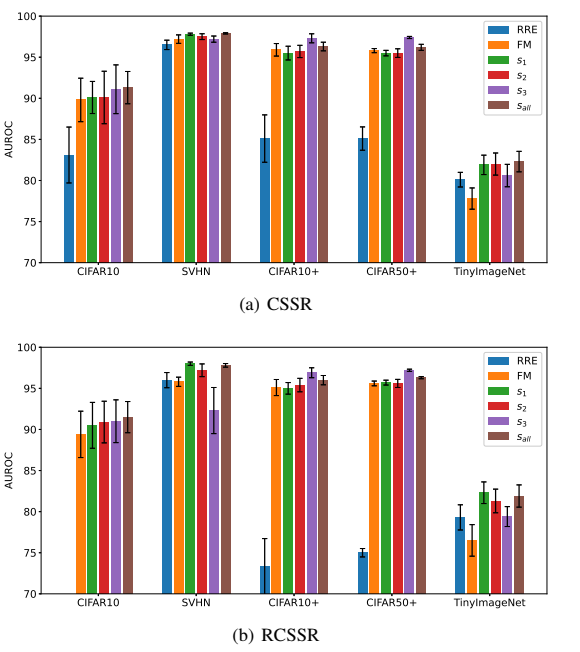
\includegraphics[width=0.48\textwidth]{fig7.png}
     \caption{The performance of individual score function in the unknown detection experiment. Note the standard deviations are calculated by the five randomized trials under different known-unknown splits} \label{fig5}
    
  \end{figure}
  In Fig. ~\ref{fig5}, we further illustrate the performance variations of different score functions in the unknown detection experiment (Table 1), showcasing how each function performs under different dataset conditions. For instance, s3 exhibits an advantage in CIFAR+10 and CIFAR+50 but not in SVHN and TinyImageNet. Nonetheless, the fused score consistently ranks at least second best with minimal standard deviation.
\subsection{Further Analysis}

Preserving closed-set performance holds equal significance in the realm of open set recognition. In this context, we conducted a comparison of closed-set performance on CIFAR10, ensuring fairness by disabling additional data augmentation techniques. The reported results from the original papers of the comparison methods were utilized for evaluation. Additionally, to account for implementation discrepancies, we included a baseline result obtained through our own implementation.
The experiment was carried out on CIFAR100, with 15 classes selected randomly as known classes. The number of unknown classes ranged from 15 to 85, resulting in openness levels ranging from 18\% to 49\%. The recognition performances of 16 classes (15 known classes and 1 unknown) were assessed based on classification accuracy. The outcomes are depicted in Fig. ~\ref{fig8}, highlighting CSSR's strong performance as openness increases, in contrast to a notable decline in performance observed when employing a plain linear classification layer.
\begin{figure}  
\centering
  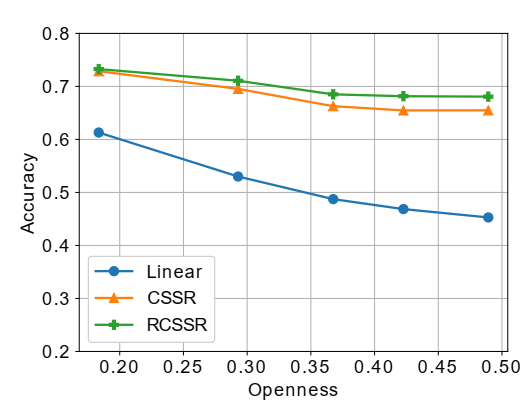
\includegraphics[width=0.48\textwidth]{fig8.png}
     \caption{Open set recognition accuracy against varying Openness for CSSR and baseline.} \label{fig8}
    
  \end{figure}
To assess our model's performance on a large-scale classification task, we conducted experiments on ImageNet-1000 \cite{10}. This dataset poses a greater challenge, comprising 1,000 classes with over one million training images and 50,000 validation images. Initially, we followed the experiment settings outlined by Yang et al. \cite{42}, selecting the first 100 classes as known and the remaining 900 as unknown. ResNet18 was chosen as the backbone network. To accommodate large-scale classification and optimize parameter usage, we reduced the dimension of the embedding space for Autoencoders (AEs) from 64 to 32. While the learning rate still commenced at 0.4, it was decreased by a factor of 10 at the 100th and 150th epochs to ensure adequate training.

Given the expanded and intricate semantic space introduced by ImageNet-1000, we disabled the representation-based score functions (w2 = w3 = 0). The remaining hyperparameters were maintained consistent with the experiments on ImageNet30. In addition to utilizing the plain linear classification layer as our baseline model, we referenced the reported results of the original prototype-based method \cite{10} for comparative analysis. It is important to note that the implementation in utilized ResNet50 as the backbone network, which is notably more robust compared to ResNet18 employed in our study.

\section{Conclusion}
In this research, we combined AE and prototype-learning frameworks to introduce a new end-to-end deep network named CSSR for open set recognition. CSSR assigns an individual AE to each known class instead of using class-specific point sets in traditional prototype learning. These AEs are added on top of the backbone DNN to reconstruct the semantic representations of the images. The class-specific AEs function as prototype learning with class-specific learnable AE manifold represented point sets. We observed that the MSE distance, commonly used in prototype learning, may lead to inconsistent distribution between prototype points and the ground-truth data distribution. To tackle this issue, we replaced MSE with MAE distance to ensure consistency between prototype points and data points. Additionally, our framework can be adapted to RCSSR with reciprocal point learning concept. By enhancing feature representations, various representation-based score functions such as first-order and second-order statistics were explored. Experimental results across multiple datasets show that our proposed method surpasses other state-of-the-art methods. Notably, CSSR requires no additional loss beyond the discriminative classification loss and functions as a classifier, making it easily extendable with different classification techniques. Dealing with high-dimensional and large-scale images poses challenges for OSR in real-world applications. Our future focus will be on addressing open set recognition with class hierarchical structures. Furthermore, our work does not currently address training an open set classifier with known outliers, which we plan to address by leveraging image backgrounds in future research.

% the part of references

\begin{thebibliography}{}
\bibitem[\protect\citename 5]{5} [1] T. Chen, S. Kornblith, M. Norouzi, and G. Hinton, “A simple frameworkfor contrastive learning of visual representations,” in ICML 2020: 37th International Conference on Machine Learning, vol. 1, 2020, pp. 1597– 1607.
   \bibitem[\protect\citename 6]{6} [2] X. Chen and K. He, “Exploring simple siamese representation learning,”in Proceedings of the IEEE/CVF Conference on Computer Vision and Pattern Recognition, 2021, pp. 15 750–15 758.
   \bibitem[\protect\citename 7]{7} [3] X. Chu, Y. Lin, X. Wang, X. Gao, Q. Tong, H. Yu, and Y. Wang,“Distance metric learning with joint representation diversification,” in ICML 2020: 37th International Conference on Machine Learning, vol. 1, 2020, pp. 1962–1973.
  \bibitem[\protect\citename 8]{8} [4] E. D. Cubuk, B. Zoph, J. Shlens, and Q. V. Le, “Randaugment: Practicalautomated data augmentation with a reduced search space,” in Proceedings of the IEEE/CVF Conference on Computer Vision and Pattern Recognition Workshops, 2020, pp. 702–703.
  \bibitem[\protect\citename 9]{9} [5] A. R. Dhamija, M. Gunther, and T. E. Boult, “Reducing network ¨agnostophobia,” in Advances in Neural Information Processing Systems, vol. 31, 2018, pp. 9157–9168.
  \bibitem[\protect\citename 10]{10} [6] Hongzhi Huang, Yu Wang, Qinghua Hu “Class-Specific Semantic Reconstruction for
Open Set Recognition,” IEEE Transactions on Pattern Analysis and Machine Intelligence, 2020. 
\bibitem[\protect\citename 1]{1} [7] A. Bendale and T. Boult, “Towards open world recognition,” in 2015IEEE Conference on Computer Vision and Pattern Recognition, 2015, pp. 1893–1902.
   \bibitem[\protect\citename 2]{2} [8] A. Bendale and T. E. Boult, “Towards open set deep networks,” in 2016IEEE Conference on Computer Vision and Pattern Recognition, 2016, pp. 1563–1572.\bibitem[\protect\citename 3]{9} [3] G. Chen, P. Peng, X. Wang, and Y. Tian, “Adversarial reciprocal pointslearning for open set recognition.” IEEE Transactions on Pattern Analysis and Machine Intelligence, pp. 1–1, 2021.
   \bibitem[\protect\citename 4]{4} [10] G. Chen, L. Qiao, Y. Shi, P. Peng, J. Li, T. Huang, S. Pu, and Y. Tian,“Learning open set network with discriminative reciprocal points,” in European Conference on Computer Vision. Springer, 2020, pp. 507– 522.
\bibitem[\protect\citename 11]{11} [11] I. Golan and R. El-Yaniv, “Deep anomaly detection using geometrictransformations,” in Advances in Neural Information Processing Systems, vol. 31, 2018, pp. 9758–9769.
\bibitem[\protect\citename 12]{12} [12] J.-B. Grill, F. Strub, F. Altche, C. Tallec, P. H. Richemond, ´E. Buchatskaya, C. Doersch, B. A. Pires, Z. D. Guo, M. G. Azar, B. Piot,K. Kavukcuoglu, R. Munos, and M. Valko, “Bootstrap your own latent:A new approach to self-supervised learning,” in Advances in NeuralInformation Processing Systems, vol. 33, 2020, pp. 21 271–21 284. 
\bibitem[\protect\citename 13]{13} [13] K. He, X. Zhang, S. Ren, and J. Sun, “Deep residual learning for imagerecognition,” in 2016 IEEE Conference on Computer Vision and Pattern Recognition, 2016, pp. 770–778.
\bibitem[\protect\citename 16]{16} [14] D. Hendrycks, M. Mazeika, S. Kadavath, and D. Song, “Using selfsupervised learning can improve model robustness and uncertainty,” in Advances in Neural Information Processing Systems, vol. 32, 2019, pp. 15 663–15 674.
\bibitem[\protect\citename 17]{17} [15] G. V. Horn, O. M. Aodha, Y. Song, Y. Cui, C. Sun, A. Shepard, H. Adam,P. Perona, and S. J. Belongie, “The inaturalist species classification anddetection dataset,” 2018 IEEE/CVF Conference on Computer Vision andPattern Recognition, pp. 8769–8778, 2018. 
\bibitem[\protect\citename 14]{14} [16] D. Hendrycks, S. Basart, M. Mazeika, M. Mostajabi, J. Steinhardt, andD. Song, “A benchmark for anomaly segmentation,” arXiv: ComputerVision and Pattern Recognition, 2019.
\bibitem[\protect\citename 15]{15} [17] D. Hendrycks and K. Gimpel, “A baseline for detecting misclassified andout-of-distribution examples in neural networks,” in ICLR (Poster), 2016.
\bibitem[\protect\citename 18]{18} [18] P. R. M. Junior, R. M. Souza, R. D. Werneck, B. V. Stein, D. V. Pazinato, ´ W. R. Almeida, O. A. Penatti, R. D. Torres, and A. Rocha, “Nearest neighbors distance ratio open-set classifier,” Machine Learning, vol. 106, no. 3, pp. 359–386, 2017.
\bibitem[\protect\citename 19]{19} [19] S. Kong and D. Ramanan, “Opengan: Open-set recognition via open datageneration.” arXiv preprint arXiv:2104.02939, 2021.
\bibitem[\protect\citename 20]{20} [20] A. Krizhevsky, “Learning multiple layers of features from tiny images.”Tech Report, 2009.
\bibitem[\protect\citename 21]{21} [21] K. Lee, K. Lee, H. Lee, and J. Shin, “A simple unified frameworkfor detecting out-of-distribution samples and adversarial attacks,” in Advances in Neural Information Processing Systems, vol. 31, 2018, pp. 7167–7177.
\bibitem[\protect\citename 22]{22} [22] S. Liang, Y. Li, and R. Srikant, “Enhancing the reliability of out-ofdistribution image detection in neural networks,” in 6th International Conference on Learning Representations, 2018.
\bibitem[\protect\citename 23]{23} [23] W. Liu, X. Wang, J. D. Owens, and Y. Li, “Energy-based out-ofdistribution detection,” in Advances in Neural Information Processing Systems, vol. 33, 2020, pp. 21 464–21 475.
\bibitem[\protect\citename 24]{24} [24] L. Neal, M. L. Olson, X. Z. Fern, W.-K. Wong, and F. Li, “Open setlearning with counterfactual images.” in Proceedings of the European Conference on Computer Vision, 2018, pp. 620–635.
\bibitem[\protect\citename 25]{25} [25] Y. Netzer, T. Wang, A. Coates, A. Bissacco, B. Wu, and A. Y. Ng,“Reading digits in natural images with unsupervised feature learning,” in Neural Information Processing Systems, 2011, pp. 1–9.
\bibitem[\protect\citename 26]{26} [26] P. Oza and V. M. Patel, “C2ae: Class conditioned auto-encoder for openset recognition,” in 2019 IEEE/CVF Conference on Computer Vision and Pattern Recognition, 2019, pp. 2307–2316.
\bibitem[\protect\citename 29]{29} [27] P. Perera, R. Nallapati, and B. Xiang, “Ocgan: One-class novelty detection using gans with constrained latent representations,” in 2019IEEE/CVF Conference on Computer Vision and Pattern Recognition (CVPR), 2019, pp. 2898–2906.
\bibitem[\protect\citename 30]{30} [28] H. Pouransari and S. Ghili, “Tiny imagenet visual recognition challenge,”CS 231N, 2014.
\bibitem[\protect\citename 31]{31} [29] I. M. Quintanilha, R. de M. E. Filho, J. Lezama, M. Delbracio, andL. O. Nunes, “Detecting out-of-distribution samples using low-order deepfeatures statistics,” 2018.
\bibitem[\protect\citename 32]{32} [30] O. Russakovsky, J. Deng, H. Su, J. Krause, S. Satheesh, S. Ma, Z. Huang,A. Karpathy, A. Khosla, M. Bernstein, A. C. Berg, and L. Fei-Fei, “Imagenet large scale visual recognition challenge,” International Journal ofComputer Vision, vol. 115, no. 3, pp. 211–252, 2015 
\bibitem[\protect\citename 27]{27} [31] robbie Stewart, “Deep cnn-based multi-task learning for open-set recognition.” arXiv preprint arXiv:1903.03161, 2019.
\bibitem[\protect\citename 28]{28} [32] P. Perera, V. I. Morariu, R. Jain, V. Manjunatha, C. Wigington, V. Ordonez, and V. M. Patel, “Generative-discriminative feature representations for open-set recognition,” in 2020 IEEE/CVF Conference on Computer Vision and Pattern Recognition (CVPR), 2020, pp. 11 814– 11 823.
\bibitem[\protect\citename 33]{33} [33] C. S. Sastry and S. Oore, “Detecting out-of-distribution examples withgram matrices,” in ICML 2020: 37th International Conference on Machine Learning, vol. 1, 2020, pp. 8491–8501.
\bibitem[\protect\citename 34]{34} [34] W. J. Scheirer, A. de Rezende Rocha, A. Sapkota, and T. E. Boult, “Toward open set recognition,” IEEE Transactions on Pattern Analysis and Machine Intelligence, vol. 35, no. 7, pp. 1757–1772, 2013.
\bibitem[\protect\citename 35]{35} [35] V. Sehwag, M. Chiang, and P. Mittal, “Ssd: A unified framework forself-supervised outlier detection,” in ICLR 2021: The Ninth International Conference on Learning Representations, 2021.
\bibitem[\protect\citename 36]{36} [36] X. Sun, Z. Yang, C. Zhang, K.-V. Ling, and G. Peng, “Conditional gaussian distribution learning for open set recognition,” in 2020 IEEE/CVF Conference on Computer Vision and Pattern Recognition, 2020, pp.13 480–13 489.
\bibitem[\protect\citename 37]{37} [37] X. Sun, C. Zhang, G. Lin, and K. V. Ling, “Open set recognition with conditional probabilistic generative models.” arXiv preprint arXiv:2008.05129, 2020.
\bibitem[\protect\citename 38]{38} [38] J. Tack, S. Mo, J. Jeong, and J. Shin, “Csi: Novelty detection viacontrastive learning on distributionally shifted instances,” in Advances in Neural Information Processing Systems, vol. 33, 2020, pp. 11 839– 11 852.
\bibitem[\protect\citename 39]{39} [39] Y. Tian, C. Sun, B. Poole, D. Krishnan, C. Schmid, and P. Isola,“What makes for good views for contrastive learning,” arXiv preprint arXiv:2005.10210, 2020.
\bibitem[\protect\citename 40]{40} [40] A. Vyas, N. Jammalamadaka, X. Zhu, D. Das, B. Kaul, and T. L. Willke,“Out-of-distribution detection using an ensemble of self supervised leaveout classifiers,” in Proceedings of the European Conference on Computer Vision (ECCV), 2018, pp. 560–574.
\bibitem[\protect\citename 41]{41} [41] J. Winkens, R. Bunel, A. G. Roy, R. Stanforth, V. Natarajan, J. R.Ledsam, P. MacWilliams, P. Kohli, A. Karthikesalingam, S. Kohl, A. T. Cemgil, S. M. A. Eslami, and O. Ronneberger, “Contrastive training for improved out-of-distribution detection.” arXiv preprint arXiv:2007.05566, 2020.
\bibitem[\protect\citename 42]{42} [42] H. M. Yang, X. Y. Zhang, F. Yin, Q. Yang, and C. L. Liu, “Convolutionalprototype network for open set recognition,” IEEE Transactions on Pattern Analysis and Machine Intelligence, in press.
\bibitem[\protect\citename 10]{43} [43] R. Yoshihashi, W. Shao, R. Kawakami, S. You, M. Iida, and T. Naemura, “Classification-reconstruction learning for open-set recognition,” in Proceedings of the IEEE Conference on Computer Vision and Pattern Recognition, 2019, pp. 4016–4025.
\bibitem[\protect\citename 44]{44} [44] F. Yu, Y. Zhang, S. Song, A. Seff, and J. Xiao, “Lsun: Construction of alarge-scale image dataset using deep learning with humans in the loop,” arXiv preprint arXiv:1506.03365, 2015.
\bibitem[\protect\citename 45]{45} [45] S. Zagoruyko and N. Komodakis, “Wide residual networks,” in BritishMachine Vision Conference 2016, 2016.
\bibitem[\protect\citename 46]{46} [46] H. Zhang and V. M. Patel, “Sparse representation-based open set recognition,” IEEE Transactions on Pattern Analysis and Machine Intelligence, vol. 39, no. 8, pp. 1690–1696, 2017.
\bibitem[\protect\citename 47]{47} [47] H. Zhang, A. Li, J. Guo, and Y. Guo, “Hybrid models for open set
\bibitem[\protect\citename 48]{48} [48] D.-W. Zhou, H.-J. Ye, and D.-C. Zhan, “Learning placeholders foropen-set recognition,” in Proceedings of the IEEE/CVF Conference on Computer Vision and Pattern Recognition, 2021, pp. 4401–4410.[49] E. Zisselman and A. Tamar, “Deep residual flow for novelty detection.”2020. 

  
  
   
\end{thebibliography}


\appendix



\end{document}
